%%%%%%%%%%%%%%%%%%%%%%%%%%%%%%%%%%%%%%%%%%%%%%%%%%%%%%%%%%%%%%%%%%%%%%
% LaTeX Example: Project Report
%
% Source: http://www.howtotex.com
%
% Feel free to distribute this example, but please keep the referral
% to howtotex.com
% Date: March 2011 
% 
%%%%%%%%%%%%%%%%%%%%%%%%%%%%%%%%%%%%%%%%%%%%%%%%%%%%%%%%%%%%%%%%%%%%%%
% How to use writeLaTeX: 
%
% You edit the source code here on the left, and the preview on the
% right shows you the result within a few seconds.
%
% Bookmark this page and share the URL with your co-authors. They can
% edit at the same time!
%
% You can upload figures, bibliographies, custom classes and
% styles using the files menu.
%
% If you're new to LaTeX, the wikibook is a great place to start:
% http://en.wikibooks.org/wiki/LaTeX
%
%%%%%%%%%%%%%%%%%%%%%%%%%%%%%%%%%%%%%%%%%%%%%%%%%%%%%%%%%%%%%%%%%%%%%%
% Edit the title below to update the display in My Documents
%\title{Project Report}
%
%%% Preamble
\documentclass[paper=a4, fontsize=11pt]{scrartcl}
\usepackage[T1]{fontenc}
\usepackage{fourier}

\usepackage[english]{babel}															% English language/hyphenation
\usepackage[protrusion=true,expansion=true]{microtype}	
\usepackage{amsmath,amsfonts,amsthm} % Math packages
\usepackage[pdftex]{graphicx}	
\usepackage{titlesec}
\usepackage{listings}
\usepackage{hyperref}
\usepackage[nameinlink,noabbrev]{cleveref}

\usepackage{xcolor}
\hypersetup{
    colorlinks,
    linkcolor={red!50!black},
    citecolor={blue!50!black},
    urlcolor={blue!80!black}
}

%% \usepackage{chngcntr}
%% \counterwithin{figure}{section}


%%% Custom headers/footers (fancyhdr package)
\usepackage{fancyhdr}
\pagestyle{fancyplain}
\fancyhead{}											% No page header
\fancyfoot[L]{}											% Empty 
\fancyfoot[C]{}											% Empty
\fancyfoot[R]{\thepage}									% Pagenumbering
\renewcommand{\headrulewidth}{0pt}			% Remove header underlines
\renewcommand{\footrulewidth}{0pt}				% Remove footer underlines
\setlength{\headheight}{13.6pt}
\usepackage[margin=0.5in]{geometry}

%%% Equation and float numbering
\numberwithin{equation}{section}		% Equationnumbering: section.eq#
\numberwithin{figure}{section}			% Figurenumbering: section.fig#
\numberwithin{table}{section}				% Tablenumbering: section.tab#

%% Section Format
\titleformat*{\section}{\LARGE\bfseries}
\titleformat*{\subsection}{\Large\bfseries}
\titleformat*{\subsubsection}{\large\bfseries}
\titleformat*{\paragraph}{\large\bfseries}
\titleformat*{\subparagraph}{\large\bfseries}
\graphicspath{ {./imgs/} }



%%% Maketitle metadata
\newcommand{\horrule}[1]{\rule{\linewidth}{#1}} 	% Horizontal rule

\title{
		%\vspace{-1in} 	
		\usefont{OT1}{bch}{b}{n}
		\normalfont \normalsize \textsc{University of Purdue\\
      Data Communication and Computer Networks\\
      CS 53600 Fall 2019} \\ [25pt]
		\horrule{0.5pt} \\[0.4cm]
		\huge Assignment 6\\
		\horrule{2pt} \\[0.5cm]
}
\author{
  \normalfont\normalsize Hanjing Xu (xu675)\\ [-5pt]
    \normalfont\normalsize Pedro da Costa Abreu (pdacost)\\[-5pt]
    \normalsize \today
  }
\date{}


%%% Begin document
\begin{document}
\maketitle

\section[1]{Problem 1}

During testing of our program we ran tests cases using the parameters: payload
size 1488 bytes, initial lambda of 90msec, gamma of 313msec, buffer size of 48
KB and target buffer occupancy of 24 KB.

We set the server on \texttt{data.cs.purdue.edu} and the client on
\texttt{escher01.cs.purdue.edu}, more specifically running the following two
commands:

\begin{lstlisting}[language=bash, breaklines=true]
./streamerd 3344 1488 11 $TMODE $FILE_sender_$TMODE.txt
./playaudio 128.10.2.13 3344 /tmp/$USER/$FILE.au 4096 3 49152 24576 $FILE_receiver_$TMODE.txt
\end{lstlisting}

where \lstinline{$FILE} is the file being transferred, and \lstinline{$TMODE} is
the transfer method A, B, C or D. All of these generated log files can be found
in \texttt{lab6/v1/logs}.

For each method we set the control parameters on the file
\texttt{control-param.dat} with the following format:

\begin{lstlisting}[mathescape=true]
  $\alpha$, $\delta$, $\varepsilon$, $\beta$
\end{lstlisting}

We began the experiment with $\alpha = 0.1$, $\delta = 0.5$,
$\varepsilon = 0.1$ and $\beta = 0.25$, but $\varepsilon$ was too
high when running experiment C, causing the transmission to end
too early due to a collapse on $\lambda$. We then fix the problem
by setting $\varepsilon = 0.05$.

Next, we run each mode for the provided files \texttt{pp.au} and \texttt{klyne-jarrett.au},
and plot all of the runs using gnuplot.

For each run we listen to check for the quality of the stream,
and we conclude that the only that is entirely faithful is method D.
Method A playback rate accelerates when lambda is too high, and then
decelerate when lambda grows back down. Method B behaves similarly
with the difference that it decelerate faster. Method C is the
worse of them because the playback rate fluctuates too much,
making the sound faster and slow all too often.


The data plot for the transfer of the file \texttt{pp.au} on the sender side
for methods A, B, C, and D are, respectfully, the following:
\autoref{fig:ppsenderA},
\autoref{fig:ppsenderB}
\autoref{fig:ppsenderC}
\autoref{fig:ppsenderD}
Then we put them all together for a better visualization on
\autoref{fig:ppsender}

Simililarly, on the receiver side we have:
\autoref{fig:ppreceiverA},
\autoref{fig:ppreceiverB},
\autoref{fig:ppreceiverC},
\autoref{fig:ppreceiverD},
\autoref{fig:ppreceiver}.

For the big file \texttt{klyne-jarrett.au} we have the plots on the same style.
\autoref{fig:jarretsenderA},
\autoref{fig:jarretsenderB},
\autoref{fig:jarretsenderC},
\autoref{fig:jarretsenderD},
\autoref{fig:jarretsender},
\autoref{fig:jarretreceiverA},
\autoref{fig:jarretreceiverB},
\autoref{fig:jarretreceiverC},
\autoref{fig:jarretreceiverD},
\autoref{fig:jarretreceiver}.

As we can see all the programs runs as expected from the discussions
in class.

This assignment was a joint effort between Hanjing and Pedro,
the workload distribution was the following: The infrastructure
was implemented as pair programming; Hanjing implemented methods
A, B, C, D, and polished the usability; Pedro implemented the
log system and plotted the graphs.

\begin{figure}[h]
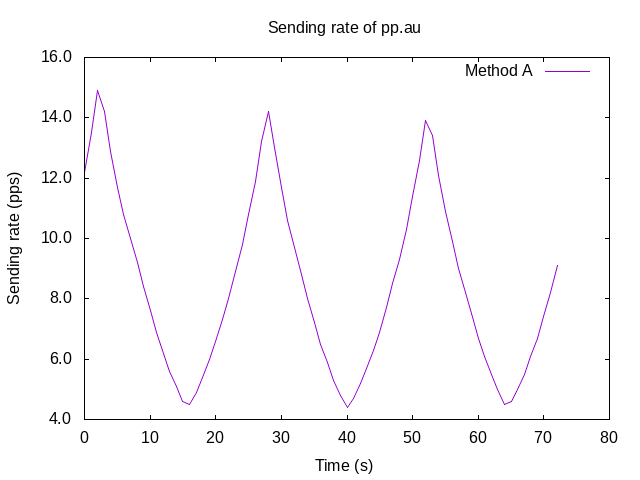
\includegraphics[width=\textwidth]{pp_sender_A}
\centering
\caption{Sending rate of pp.au for method A}
\label{fig:ppsenderA}
\end{figure}

\begin{figure}[h]
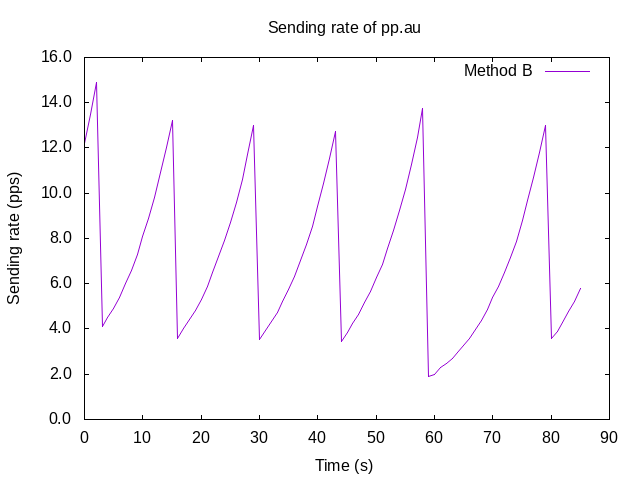
\includegraphics[width=\textwidth]{pp_sender_B}
\centering
\caption{Sending rate of pp.au for method B}
\label{fig:ppsenderB}
\end{figure}

\begin{figure}[h]
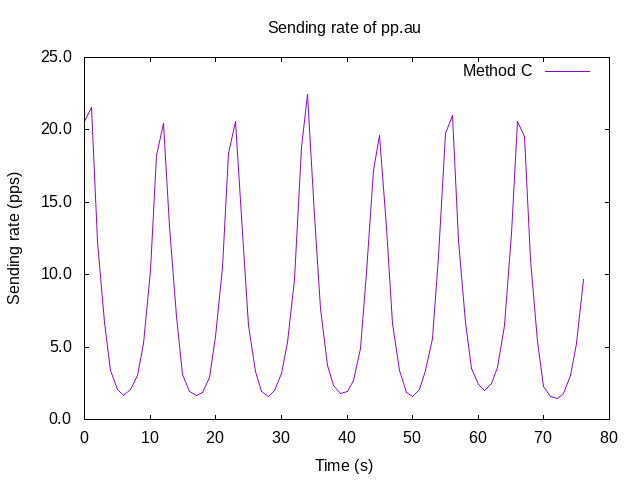
\includegraphics[width=\textwidth]{pp_sender_C}
\centering
\caption{Sending rate of pp.au for method B}
\label{fig:ppsenderC}
\end{figure}

\begin{figure}[h]
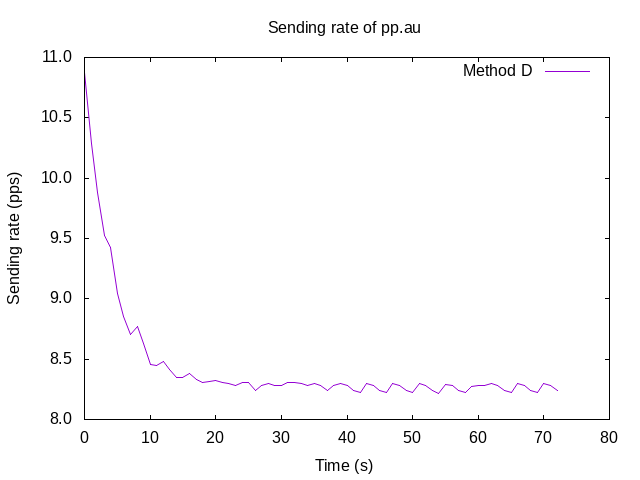
\includegraphics[width=\textwidth]{pp_sender_D}
\centering
\caption{Sending rate of pp.au for method D}
\label{fig:ppsenderD}
\end{figure}

\begin{figure}[h]
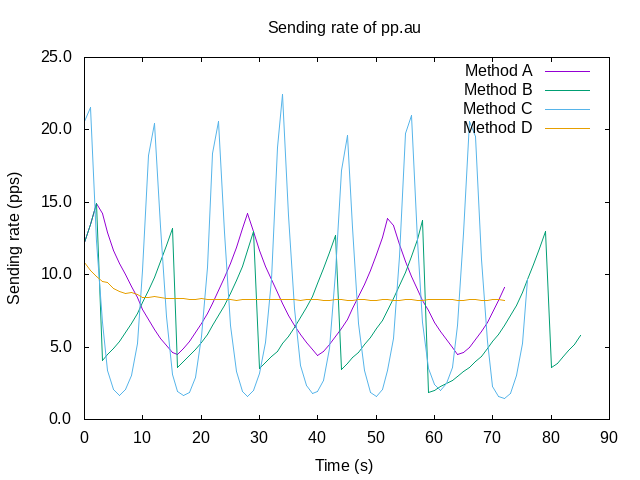
\includegraphics[width=\textwidth]{pp_sender}
\centering
\caption{Sending rate of pp.au for all methods}
\label{fig:ppsender}
\end{figure}

\begin{figure}[h]
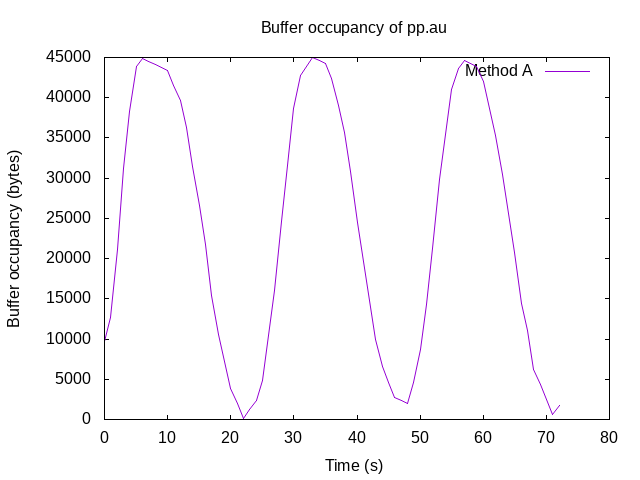
\includegraphics[width=\textwidth]{pp_receiver_A}
\centering
\caption{Buffer occupancy rate for method A}
\label{fig:ppreceiverA}
\end{figure}

\begin{figure}[h]
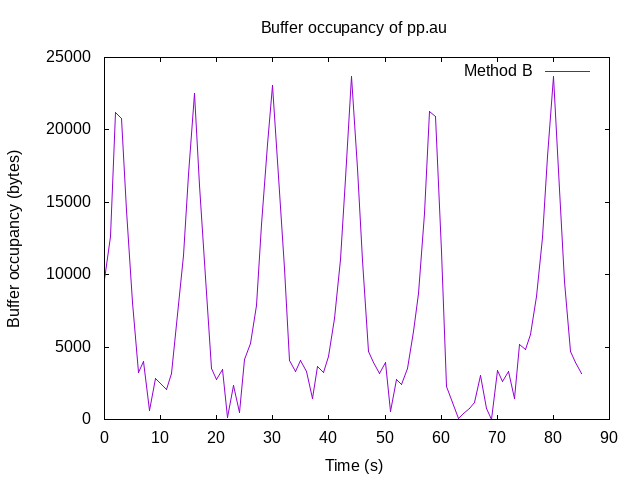
\includegraphics[width=\textwidth]{pp_receiver_B}
\caption{Buffer occupancy rate for method B}
\label{fig:ppreceiverB}
\centering
\end{figure}

\begin{figure}[h]
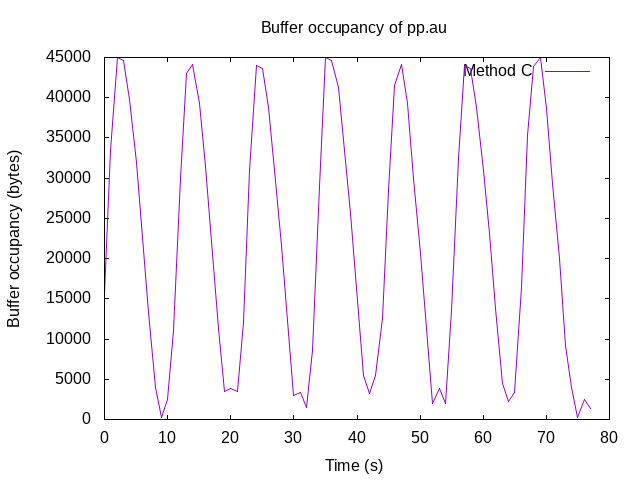
\includegraphics[width=\textwidth]{pp_receiver_C}
\caption{Buffer occupancy rate for method C}
\label{fig:ppreceiverC}
\centering
\end{figure}

\begin{figure}[h]
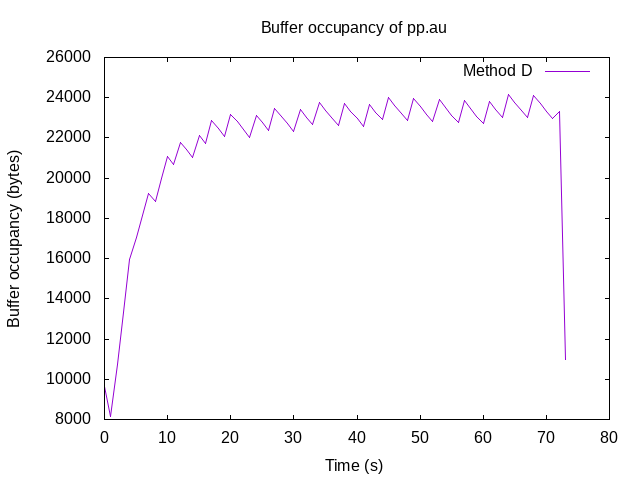
\includegraphics[width=\textwidth]{pp_receiver_D}
\caption{Buffer occupancy rate for method D}
\label{fig:ppreceiverD}
\centering
\end{figure}

\begin{figure}[h]
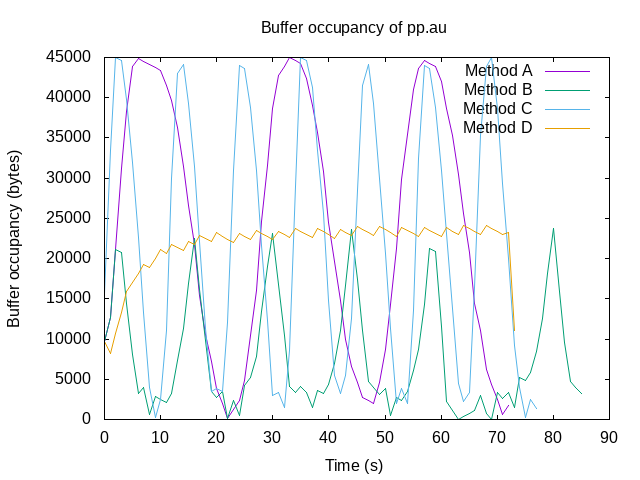
\includegraphics[width=\textwidth]{pp_receiver}
\caption{Buffer occupancy rate for all methods}
\label{fig:ppreceiver}
\centering
\end{figure}


\begin{figure}[h]
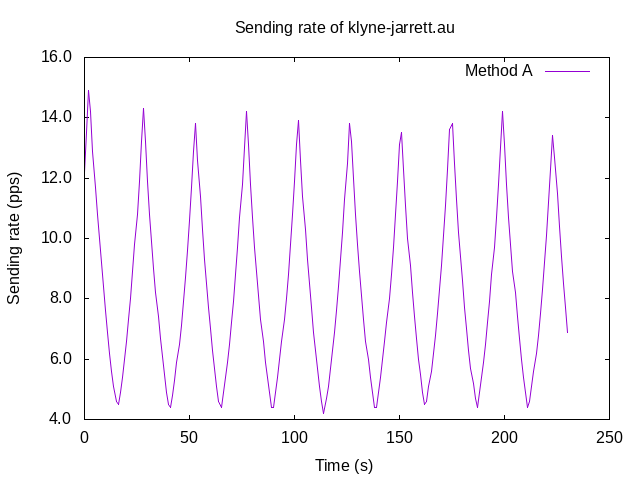
\includegraphics[width=\textwidth]{jarret_sender_A}
\caption{Sending rate for method A}
\label{fig:jarretsenderA}
\centering
\end{figure}

\begin{figure}[h]
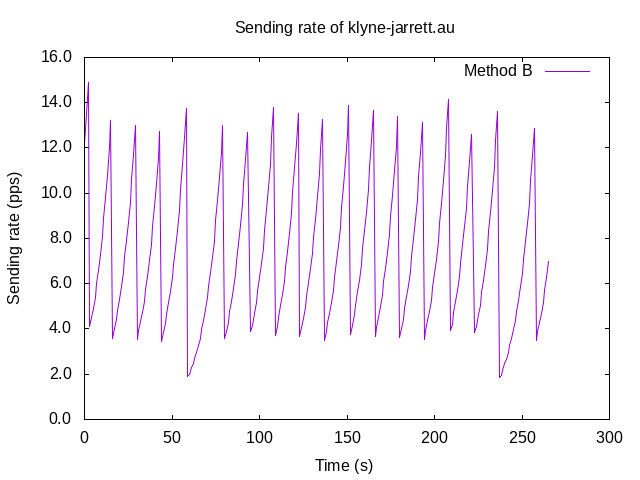
\includegraphics[width=\textwidth]{jarret_sender_B}
\caption{Sending rate for method B}
\label{fig:jarretsenderB}
\centering
\end{figure}

\begin{figure}[h]
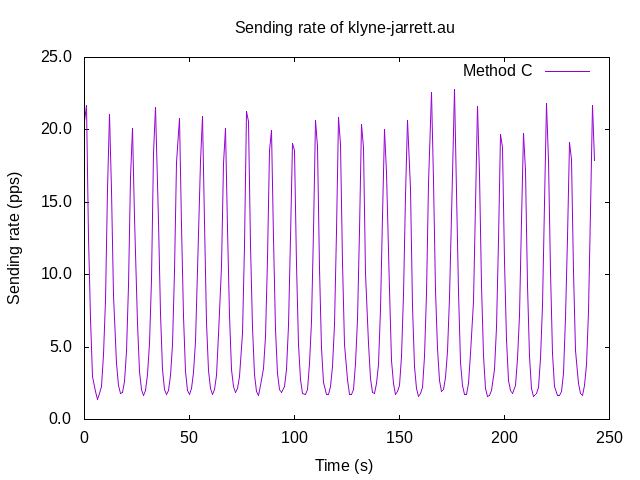
\includegraphics[width=\textwidth]{jarret_sender_C}
\caption{Sending rate for method C}
\label{fig:jarretsenderC}
\centering
\end{figure}

\begin{figure}[h]
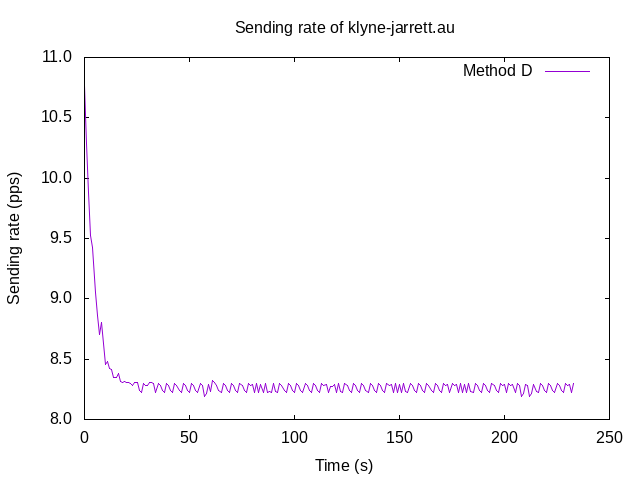
\includegraphics[width=\textwidth]{jarret_sender_D}
\caption{Sending rate for method D}
\label{fig:jarretsenderD}
\centering
\end{figure}

\begin{figure}[h]
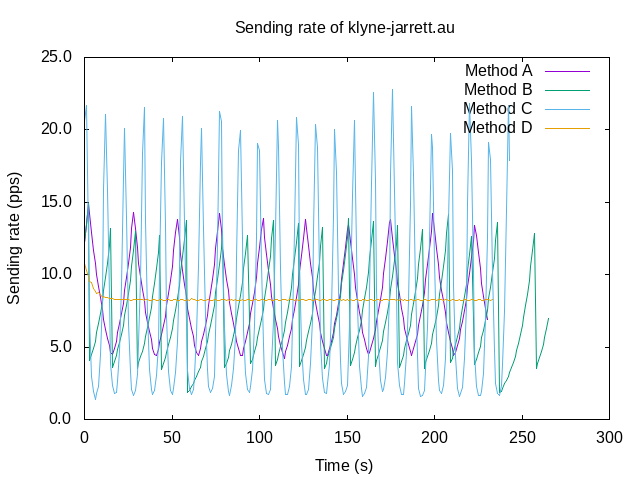
\includegraphics[width=\textwidth]{jarret_sender}
\caption{Sending rate for all methods}
\label{fig:jarretsender}
\centering
\end{figure}



\begin{figure}[h]
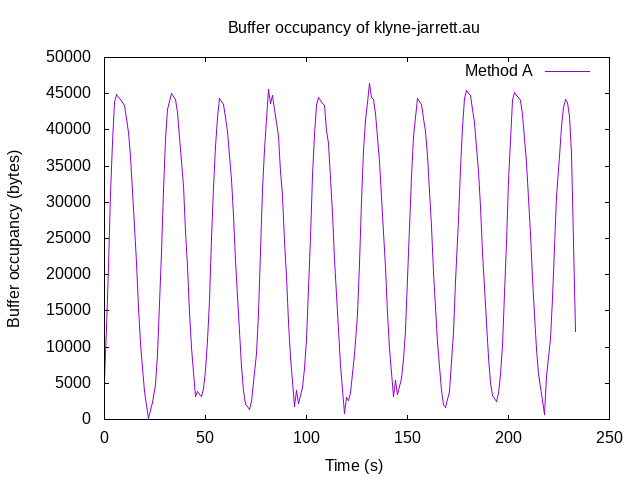
\includegraphics[width=\textwidth]{jarret_receiver_A}
\caption{Buffer occupancy rate for method A}
\label{fig:jarretreceiverA}
\centering
\end{figure}

\begin{figure}[h]
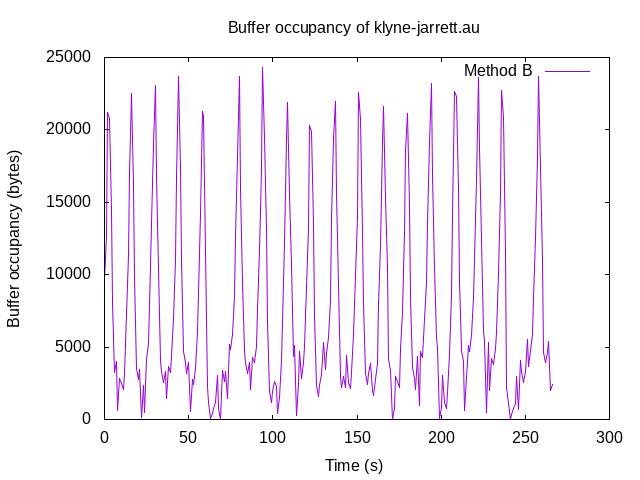
\includegraphics[width=\textwidth]{jarret_receiver_B}
\caption{Buffer occupancy rate for method B}
\label{fig:jarretreceiverB}
\centering
\end{figure}

\begin{figure}[h]
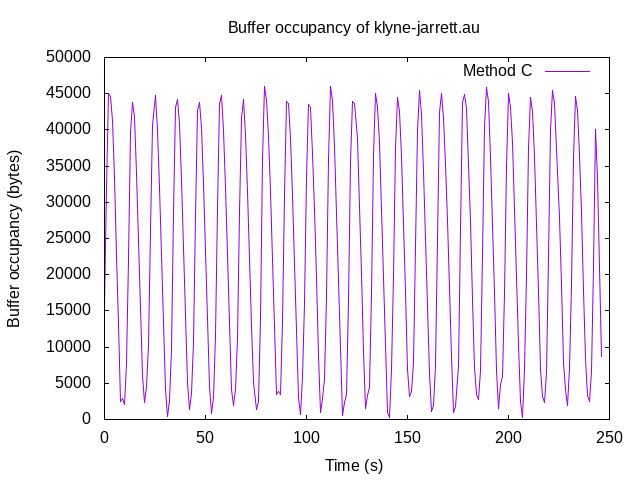
\includegraphics[width=\textwidth]{jarret_receiver_C}
\caption{Buffer occupancy rate for method C}
\label{fig:jarretreceiverC}
\centering
\end{figure}

\begin{figure}[h]
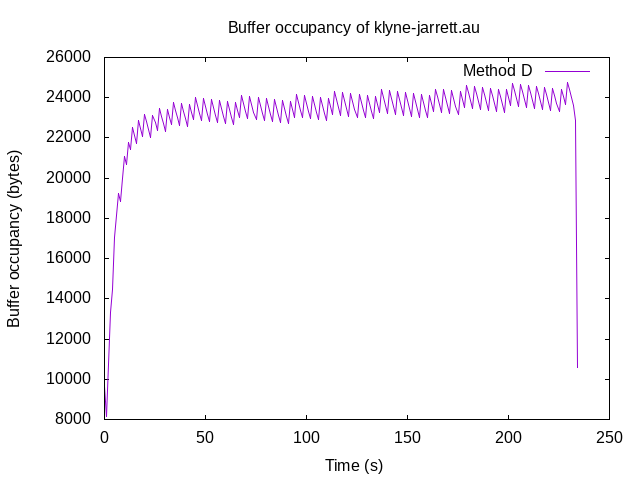
\includegraphics[width=\textwidth]{jarret_receiver_D}
\caption{Buffer occupancy rate for method D}
\label{fig:jarretreceiverD}
\centering
\end{figure}

\begin{figure}[h]
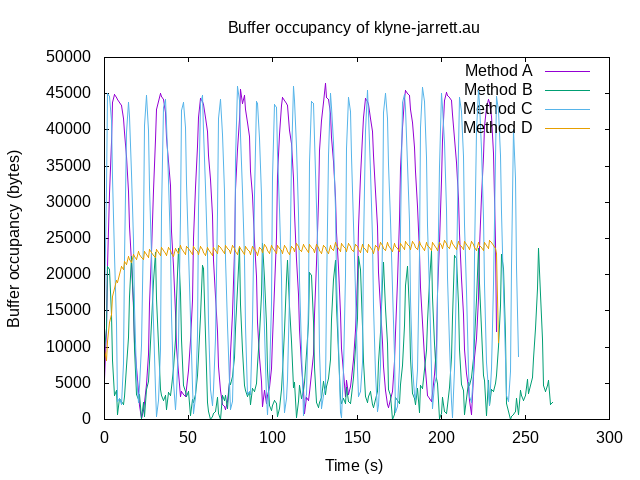
\includegraphics[width=\textwidth]{jarret_receiver}
\caption{Buffer occupancy rate for all methods}
\label{fig:jarretreceiver}
\centering
\end{figure}

%%% End document
\end{document}
